\documentclass[11pt]{scrartcl}

% standard packages
\usepackage[utf8]{inputenc}  % input in UTF-8
\usepackage[T1]{fontenc}  % output in T1 fonts (westeuropäische Codierung)
\usepackage{lmodern}  % latin modern fonts
\usepackage[ngerman]{babel}  % deutsches Sprachpaket, neue Rechtschreibung

% Seitensetup
\usepackage{scrlayer-scrpage}  % Seitenformatierung durch KOMA-interne Optionen
\usepackage[top=4cm, bottom=4cm]{geometry}  % Seitengeometrie (kann durch KOMA ersetzt werden, hab ich aber nicht geschafft)
\usepackage[hypcap=false]{caption, subcaption}  % caption editing - hypcap warning with hyperref
\usepackage{array}  % table editing

% additional packages
\usepackage{amsmath, amssymb, amstext}  % math packages (American Math Society)
\usepackage{bm}
\usepackage{icomma}  % Kommata in Dezimalzahlen verursachen keinen Abstand mehr
\usepackage{graphicx}  % Bilder einfügen
\usepackage{float} %Bilder placement
\usepackage{pdfpages}  % PDF als vollständige Seiten einfügen
\usepackage{lastpage}  % referenziert die letzte Seite
\usepackage[separate-uncertainty=true]{siunitx}  % bessere Darstellung von Einheiten
\usepackage{makecell} %Dicke Tabellenstriche
%\usepackage{datatool}
\usepackage[hidelinks]{hyperref}  % hyperref verlinkt Referenzen - hidelinks entfernt borders um links

% package setups
% Kopf- und Fußzeile durch KOMA
\pagestyle{scrheadings}  % KOMA darf entscheiden
\clearpairofpagestyles  % reset
\setkomafont{pageheadfoot}{\normalfont}  % Standardschrift in Kopf- und Fußzeile
\captionsetup{format=plain, font=small, labelfont=bf} %Better caption, Abbildung ist FETT
%\setlength{\headheight}{27.2pt}  % benötigte Höhe Kopfzeile (warning von scrlayer-scrpage, wird aber automatisch so gerendert, falls diese Option weggelassen wird)
\ihead{Stirlingmotor}  % Kopf links %Todo Titel ändern
\chead{\textsc{Philipp} Maximilian}  % Kopf Mitte %Todo Name ändern
\ohead{8. Mai 2021}  % Kopf rechts %Todo Datum ändern
\cfoot{\pagemark \, / \pageref{LastPage}}  % Fuß Mitte

% Table of Contents
\DeclareTOCStyleEntry{dottedtocline}{section}  % KOMA intern - Inhaltsverzeichnis mit Punkten (nur sections)

%Overbar setup
\newcommand{\overbar}[1]{\mkern 1.5mu\overline{\mkern-1.5mu#1\mkern-1.5mu}\mkern 1.5mu}
% SI
\sisetup{locale = DE}  % deutschsprachige SI-Konvention
\sisetup{quotient-mode = fraction}
\sisetup{per-mode = fraction}
\DeclareSIUnit\px{px}

% citation
\usepackage{csquotes}
\usepackage[backend=biber]{biblatex}
\addbibresource{stirling.bib} %Todo .bib befüllen zb.: mit JabRef (Empfehlung der Redaktion)

% array
\renewcommand{\arraystretch}{1.2}

\begin{document}

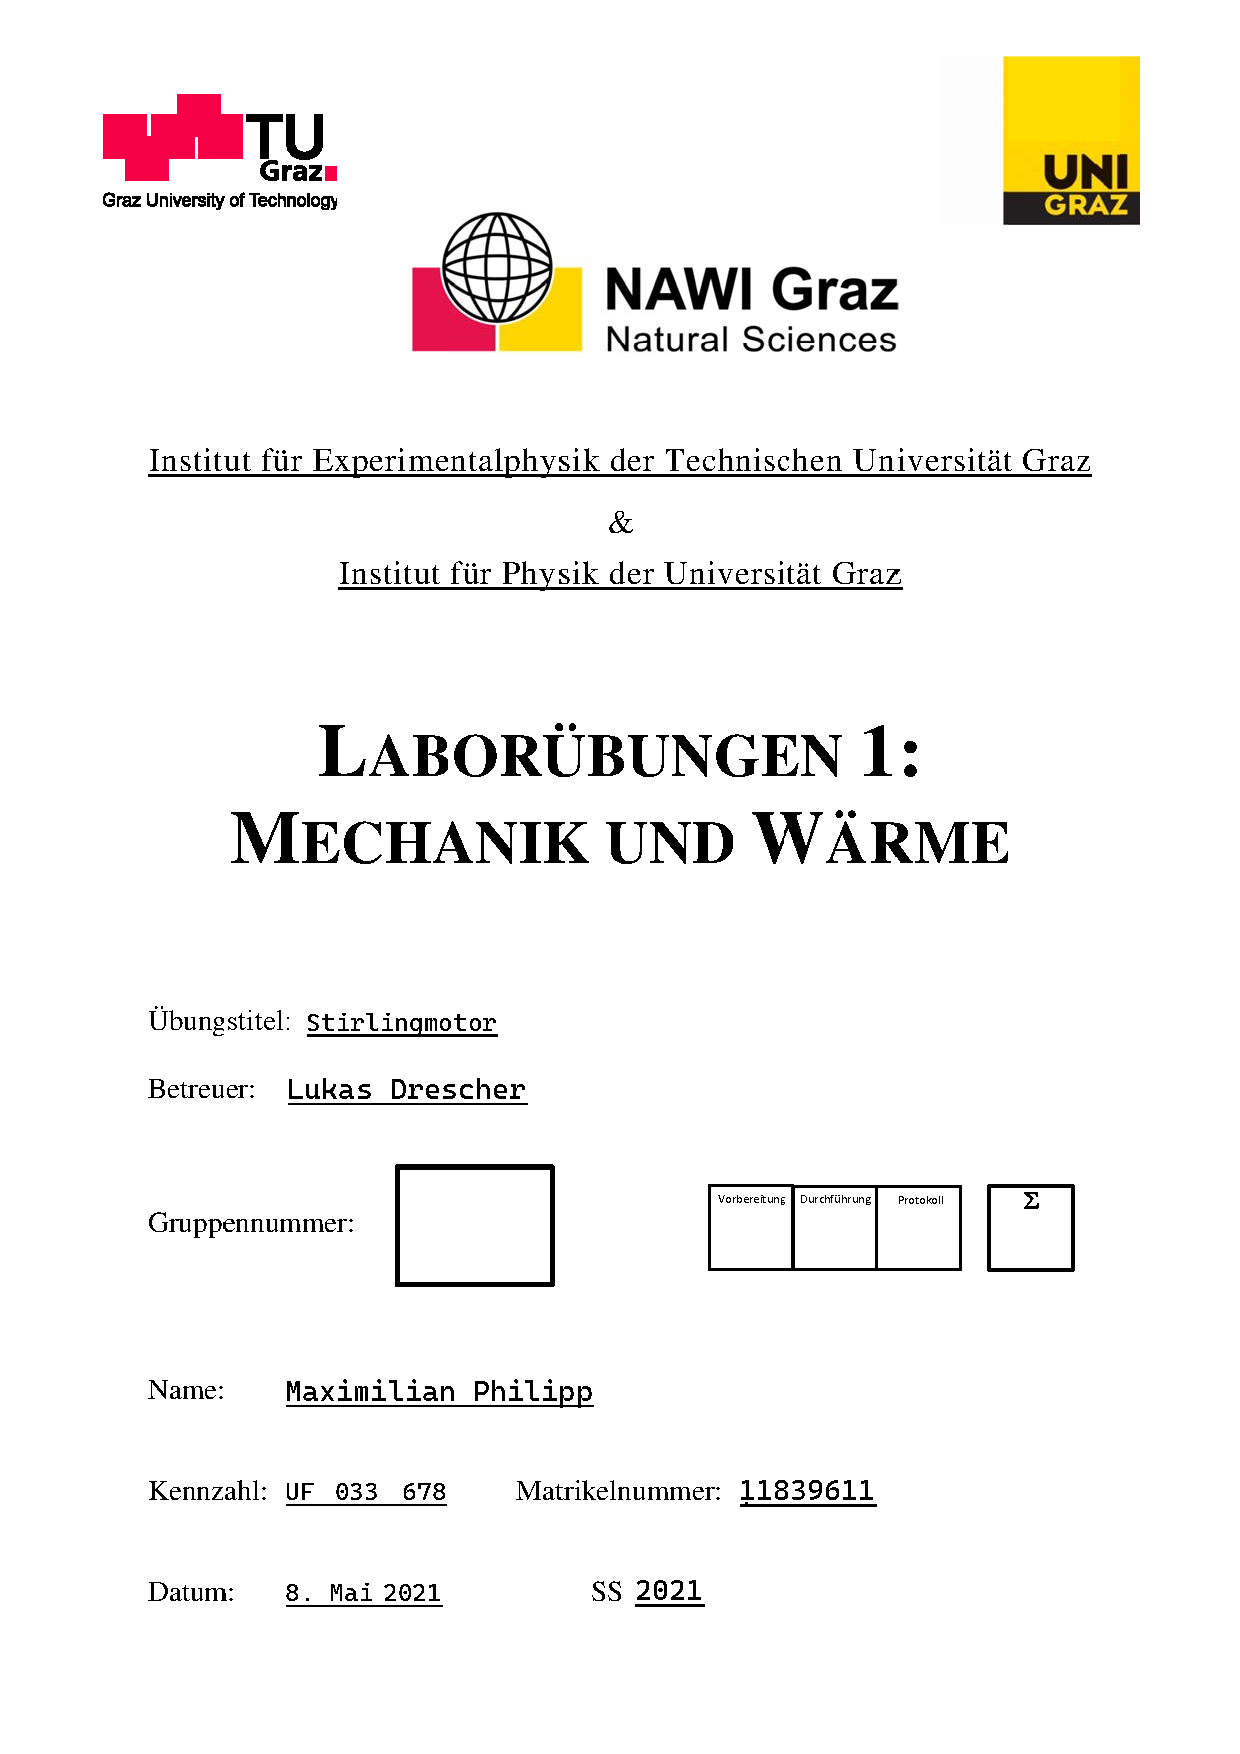
\includepdf{pdfs/Deckblatt.pdf} % Todo Deckblatt ausfüllen

\tableofcontents
\newpage
\section{Aufgabenstellung}
\label{sec:aufgabenstellung}

Die folgenden Punkte sind zu erfüllen:
\begin{itemize}
    \item Die Erstellung von $p(t)$-, $V(t)$- und $pV$-Diagrammen aus den Messdaten 
        für einen unbelasteten [1] sowie einen belasteten [2] Stirlingmotor.
    \item Berechnung der verrichteten mechanischen Arbeit $W_{\text{mech}}$ bei einem 
        Durchlauf der $pV$-Kurve durch numerische Integration.
    \item Bestimmung der mechanischen Leistung $P_{\text{mech}}$ aus der vorher 
        bestimmten mechanischen Arbeit und der Drehzahl $n$, welche sowohl
        aus dem Frequenzspektrum der Volumenschwingung durch plotten der
        gegebenen Werte $V(f)$ und der Frequenz $f$,
         als auch durch das Fitten bzw. Abzählen der Peaks pro Zeit ermittelt 
         werden kann.
     \item Berechnung des Wirkungsgrades des Stirlingmotors $\eta_{\text{L}}$.
    \item Ermittlung der über das Kühlsystem abgeführten Wärmemenge 
        $Q_{\text{ab}}$ pro Zyklus des Motors sowie der damit abgeführten
        Wärmeleistung $P_{\text{ab}}$.
    \item Die Bestimmung dieser Größen ist sowohl für den unbelasteten Betrieb
        als auch für den belasteten Betrieb des Stirlingmotors zu machen.
\end{itemize}

\section{Voraussetzungen und Grundlagen}
\label{sec:voraussetzungen_grundlagen}
Ein Stirlingmotor ist eine Wärmekraftmaschine, das bedeutet, dass sie durch
das Transportieren von Wärme einer höheren Temperaturquelle zu einer niedrigeren
für uns mechanische Arbeit vollrichten kann. Dies ist in \autoref{fig:Wärmepumpe}
veranschaulicht.

Damit dieser Motor auch nützlich sein kann muss dieser Wärmetransport so oft wie 
möglich passieren, da immer nur ein Teil der transportierten Energie in
nutzbare Arbeit umgewandelt. Die maximale theoretische Ausbeute ist durch den
Carnot Wirkungsgrad $\eta_{\text{Carnot}}$ gegeben, siehe \autoref{eq:carnot}.

\begin{equation}
    \eta_{\text{Carnot}} = 1 - \frac{T_{\text{min}}}{T_{\text{max}}} \label{eq:carnot}
\end{equation}

Wobei $T_{\text{min}}$ die Temperatur der niedrigen Temperaturquelle ist und $T_{\text{max}}$
die Temperatur der höheren Temperaturquelle ist.

Der Stirlingmotor durchgeht einen 4-teiligen Kreisprozess, bei welchem 
jedes mal, wie zuvor erwähnt, ein Teil der transportieren Wärme in 
nutzbare Arbeit umgewandelt wird. 
\begin{enumerate}
    \item Isotherme Expansion ($T=$ konst.): Das Volumen($\uparrow$) steigt 
        und der Druck($\downarrow$) fällt indem 
        der Kolben durch das Gas nach unten gedrückt wird. In diesem Schritt
        vollrichtet das Gas Arbeit.
    \item Isochore Abkühlung ($V=$ konst.): Die Temperatur($\downarrow$) 
        fällt und der Druck($\downarrow$) fällt auch indem das Gas durch die 
        niedrige Temperaturquelle abgekühlt wird.
    \item Isotherme Kompression ($T=$ konst.): Das Volumen($\downarrow$) wird kompremiert
        und der Druck($\uparrow$) steigt indem der Kolben sich nach oben beweget. In 
        diesem Schritt wird Energie benötigt.
    \item Isochore Erwärmung ($V=$ konst.): Die Temperatur($\uparrow$)
        steigt und der Druck($\uparrow$) nimmt zu indem das kompremierte Gas 
        durch die hohe Temperaturquelle erwärmt wird.
\end{enumerate}

Diese Vierzyklen, wie oben in der Aufzählung nummeriert, werden nocheinmal
in \autoref{fig:Kreisprozess_Ideal} als $pV$-Diagramm visulisiert. Die 
Fläche eingeschlossen in der Kurve ist die abgreifbare Energie pro Zyklus.

\begin{figure}[H]
    \begin{center}
        \begin{minipage}[htbp]{.4\linewidth} % [b] => Ausrichtung an \caption
            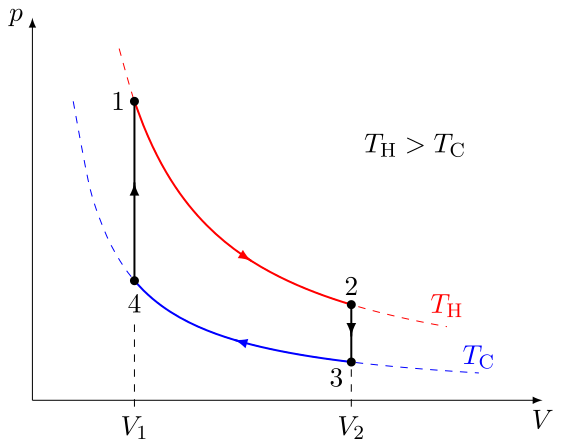
\includegraphics[width=0.925\linewidth]{pics/Stirling_cycle_pV.svg.png}
            \caption[Kreisprozess des Stirlingmotors]{Darstellung des 
            idealisierten Stirlingkreisprozess in einem $pV$-Diagramm.
            Wo $p$ der Druck und $V$ das Volumen ist.}
            \label{fig:Kreisprozess_Ideal}
        \end{minipage}
        \hspace{.1\linewidth}% Abstand zwischen Bilder
        \begin{minipage}[htbp]{.4\linewidth} % [b] => Ausrichtung an \caption
            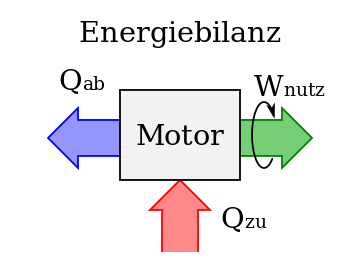
\includegraphics[width=\linewidth]{pics/Energiebilanz_Motor.svg.png}
            \caption[Wärmepumpe Darstellung]{Vereinfachte schematische 
            Darstellung einer Wärmepumpe. Hier wird veranschaulicht, dass
            nur ein Teil der zugeführten Wärmeenergie $Q_{\text{zu}}$ in Arbeit $W_{\text{nutz}}$
            umgewandelt wird. Der Rest $Q_{\text{ab}}$ wird an die niedrige Temperaturquelle
            abgegeben.}
            \label{fig:Wärmepumpe}
        \end{minipage}
    \end{center}
 \end{figure}

Jedoch ist zu erwähnen, dass die \autoref{fig:Kreisprozess_Ideal} dem  
idealisiertem Kreisprozess entspricht. Diese scharfen Kanten werden in
diesem Experiment nicht ersichtlich sein, dies wird im Kapitel \nameref{sec:diskussion_zusammenfassung}
noch genauer diskutiert.

Da die Wirkungsgrade des Systems im Mittelpunkt des Experiments stehen, muss
nur der Input und Output verglichen werden (die ins System hinzugefügte 
Leistung ($P_{\text{in}}$) und der abgreifbaren Leistung ($P_{\text{out}}$)) und nicht 
jeder Schritt des Kreisprozesses.

\begin{equation}
    \label{eq:Wirkungsgrad}
    \eta = \frac{P_{\text{out}}}{P_{\text{in}}}
\end{equation}

Um den Output des Systems zu messen gibt es verschiedene Methoden, in diesem
Experiment werden drei Methoden genutzt. 
\begin{enumerate}
    \item Durch die gemessen Daten des Volumens und des Drucks
    \item Durch Schlussrechnung mittels der im Wasser abgeführten Wärmemenge
    \item Durch Messung der abgreifbaren mechanischen Leistung $P_{\text{mech}}$ 
        mittels dem Drehmoment und der Frequenz.
\end{enumerate}

Um die abgeführte Wärmemenge pro Sekunde ($P_{\text{ab}}$) zu berechnen wurde die
\autoref{eq:Warmeleistung} \cite{dem13} an dieses Experiment angepasst. Wo $\dot V$ der
Volumenstrom, $\rho$ die Dichte des Wasser, $c$ die spezifische Wärmekapazität
von Wasser und $\Delta T$ der Temperaturanstieg durch die abgebene Wärme ist.

\begin{equation}
    \label{eq:Warmeleistung}
    P_{\text{ab}} = \dot Q_{\text{ab}} = \dot V \rho c \Delta T 
\end{equation}

Weiters wird auch $P_{\text{mech}}$, welche der Bremszaum auf die Federwaage
mittels der Kraft $F$ und dem Hebelarm $r$ pro Sekunde überträgt, durch
\autoref{eq:Drehleistung} bestimmt:

\begin{equation}
    \label{eq:Drehleistung}
    P_{\text{mech}} = F \cdot l \cdot 2 \pi f
\end{equation}

Um zu sehen wie sich die Unsicherheit der Messungen bis in die Ergebnisse 
fortplanzt, ist \autoref{eq:Unsicherheitsfortpflanzung} verwendet worden.
Die Grundlagen dieser \autoref{eq:Unsicherheitsfortpflanzung} sind von den Powerpointfolien von 
GUM entnommen worden.\cite{Kessel2004} Die Verallgemeinerung ist von Wikipedia entnommen
worden \cite{2020Fehler}.
Für die Auswertung der Unsicherheitfortpflanzung ist die Progammiersprache
Python im speziellen das Packet \verb#scipy# und \verb|sympy| für die
Aufstellung und Ausrechnung der Funktionen, zur Hilfe genommen worden.

\begin{equation}
    \label{eq:Unsicherheitsfortpflanzung}
    V_y = J(x) \cdot V_x \cdot J^{T}(x)
\end{equation}

Wobei $V_y$ und $V_x$ die Kovarianzmatrizen von den Vektoren $\bm{y}$ und $\bm{x}$.
$\bm{x}$ ist der Vektor der Eingangsvariablen und $\bm{y}$ ist der Vektor der Ausgangsvariabeln.
$J$ ist die Jakobimatrix der vektorwertigen Funktion $\bm{y} = \vec{F}(\bm{x})$ ist.
So lassen sich die Komponent der Matrix relativ einfach anschreiben $J_{ij}(x) = \frac{\partial{y_i}}{\partial{x_j}}(x)$.
Damit man die Unsicherheit der einzelnen Variabeln $y_i$ bekommt muss nur die Quadratwurzel des i-ten Diagonalelementes der 
$\bm{y}$-Kovarianzmatrix genommen werden $u_i= \sqrt{\mathrm{diag}(V_y)_i}$.
Da in diesem Experiment meistens nur skalare Funktionen untersucht werden vereinfacht
sich die \autoref{eq:Unsicherheitsfortpflanzung} dramatisch und die Unsicherheit
der Variabel $y$ lässt sich einfach so berechnen:

\begin{equation}
    \label{eq:graduncentainty}
    u_y = \sqrt{\mathrm{grad} y^T \cdot V_x \cdot \mathrm{grad} y}
\end{equation}

\section{Versuchsanordnung}
\label{sec:versuchsanordnung}
In diesem Experiment wurde eine Stirlingmotor der $\beta$-Konfiguration
verwendet. Dies bedeutet, dass die zwei Kolben in einem Zylinder sich 
bewegen, wie in \autoref{fig:Motoraufbau} ersichtlich. Da der, hier
verwendete, Stirlingmotor von der Firma LD Didavtic GmbH schon 
zusammengebaut verkauft wird, wird auf diesen Aufbau hier nicht
genauer eingegangen. Jedoch wird noch erklärt wie dieser konfiguriert
wird, damit Druck und Volumen aufgezeichnet werden kann. Zunächst
wird eine Angelschnurr benötigt um diese an die Öse des Trägers zu hängen
und über den Wegaufnehmer(b) an dem Gitter mit einer Schraubenfeder(a) zu 
befestigen. Dies möglich das Aufnehmen des Volumens im Zylinder. Weiters
wir der Drucksensor(c) mittels einem Schlauch an den inneren Hohlraum
des Zylinders geschlossen. Im obersten Teil des Motors ist die Glühwendel,
welche Wärme dem System hinzufügt. Direkt unter dieser, mit einem Gitter
umschlossenen, Kuppel ist der Anschluss für das fließende Wasser, welches
die niedrige Temperaturquelle ist.

\begin{figure}[H]
    \centering
    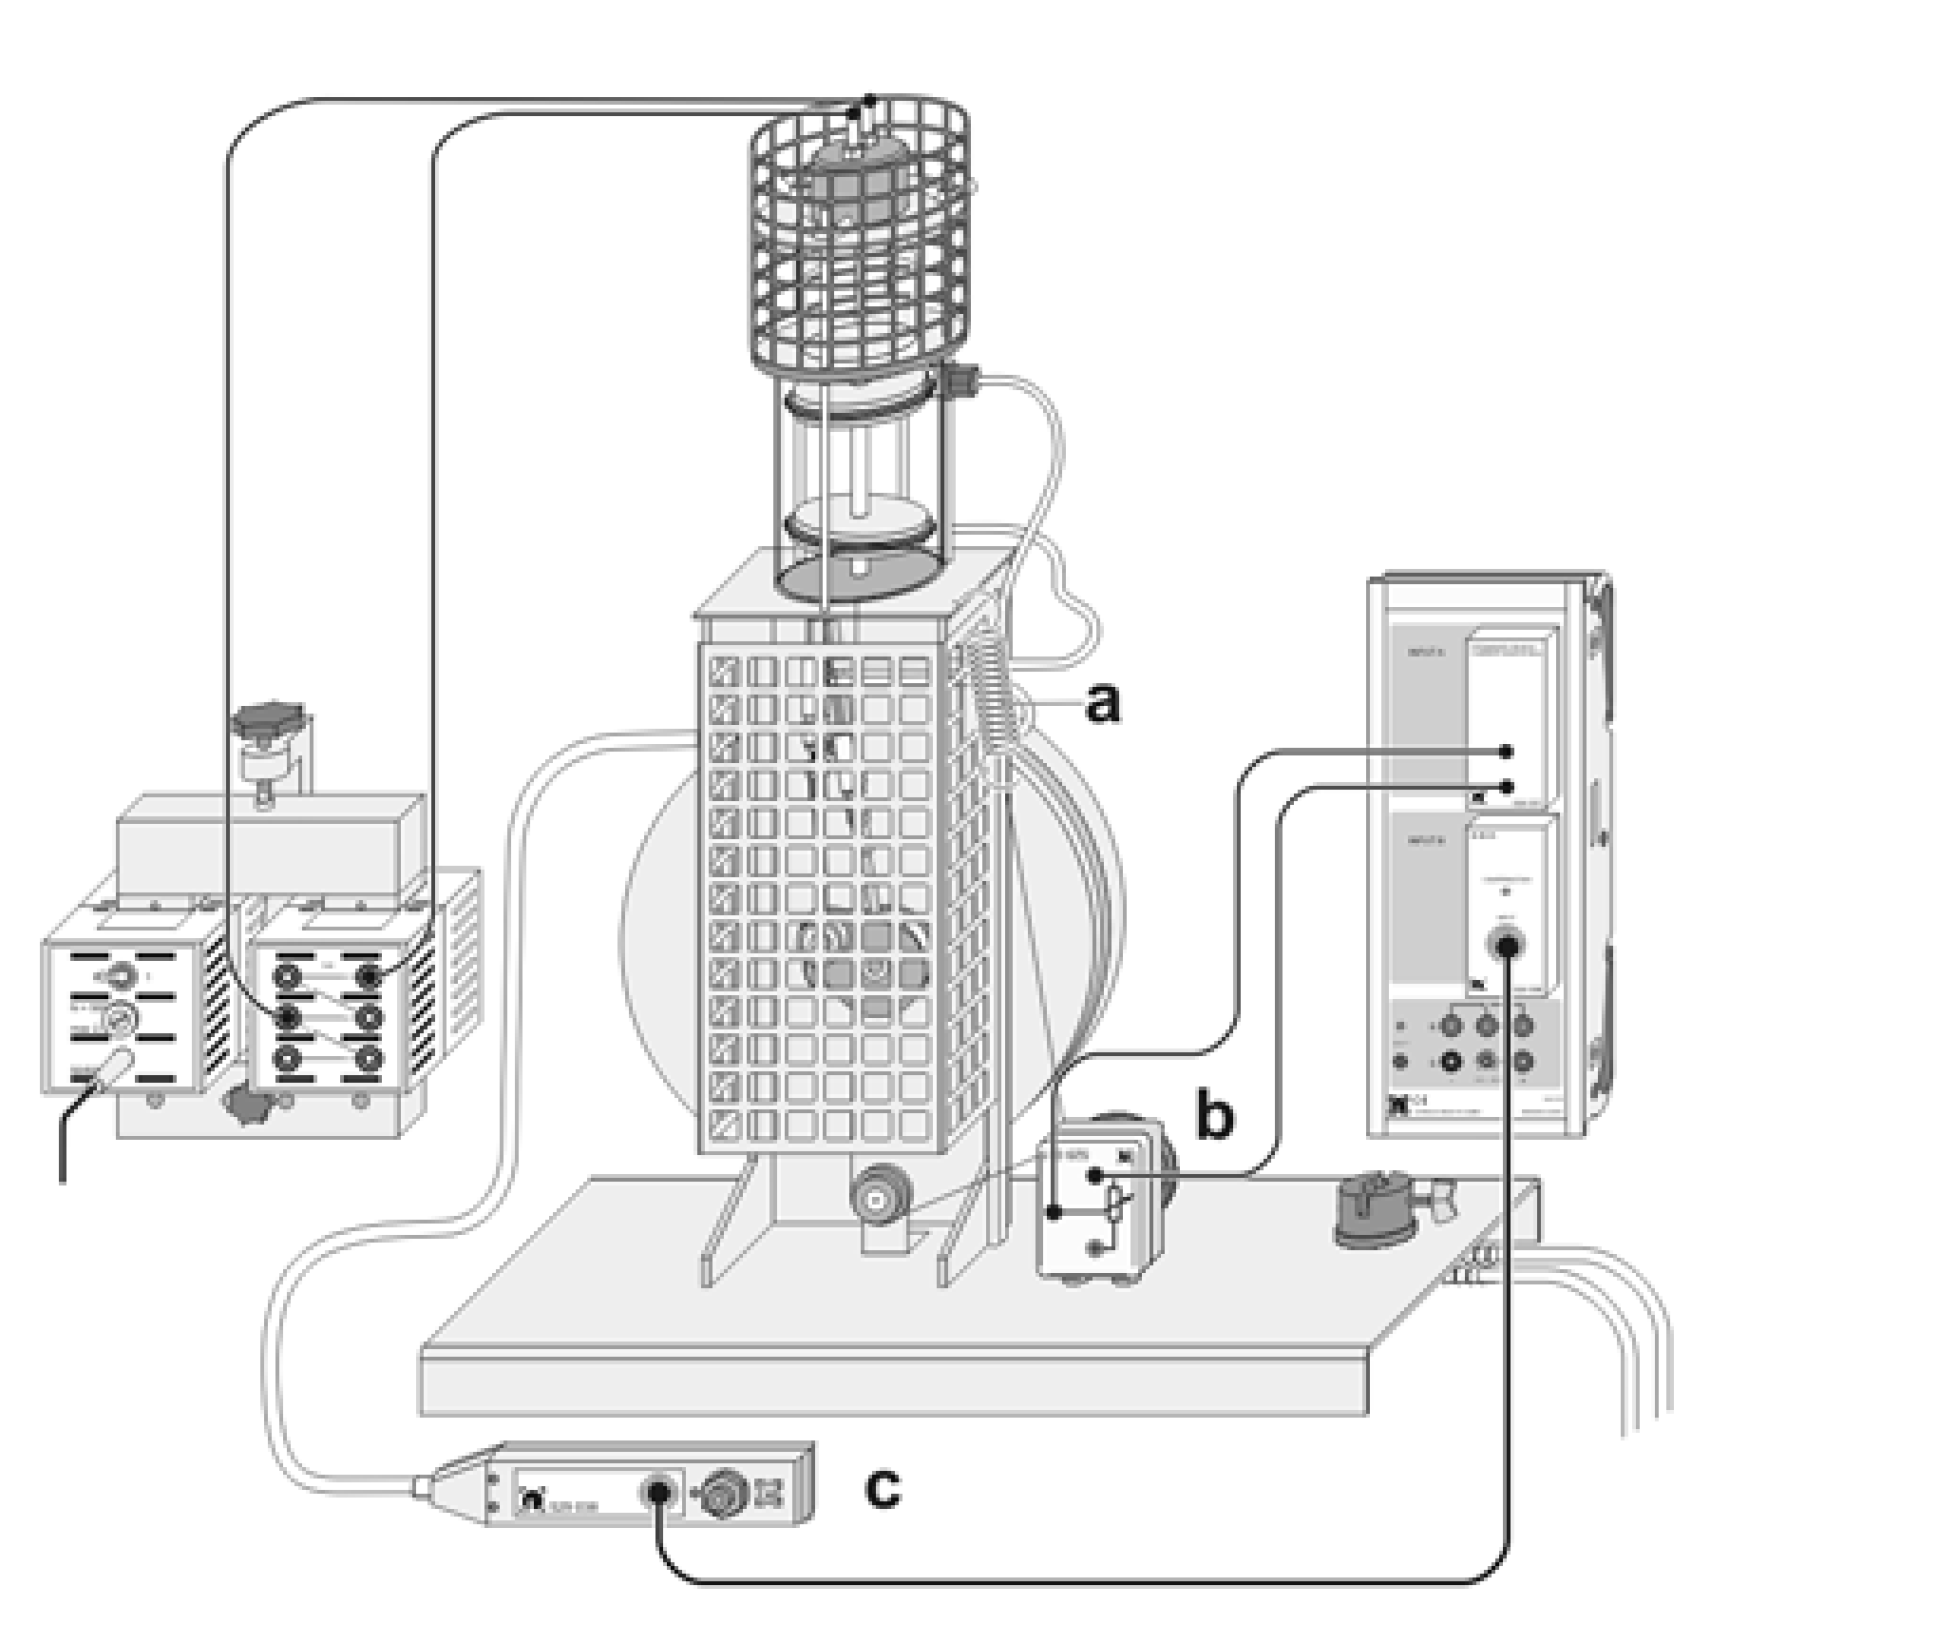
\includegraphics[width=0.8\linewidth]{pics/Motoraufbau.png}
    \caption{Aufbau des Stirlingmotors, um das Volumen und den Druck innerhalb
    des Zylinders zu messen}%
    \label{fig:Motoraufbau}
\end{figure}
% \begin{figure}[htbp] %Todo add graphic
%     \centering
%     \caption[Versuchsanordnung]{Bla Bla}
%     \label{fig:Versuchsanordnung}  % after caption for right numbering
    
%     \includegraphics[width=0.35\textwidth]{NAME.png}
% \end{figure}

\section{Geräteliste}
\label{sec:geraeteliste}
\begin{center}
    \captionof{table}[Geräteliste]{Verwendete Geräte}  % optionales Argument wird in Verzeichnissen verwendet, essentielles Argument direkt im Text
    \label{tab:geraeteliste}
    \vspace{3mm}  % vertical space 3 mm
    \hspace*{-6.0em}
    \begin{tabular}{|c|c|c|c|p{9em}|}
        \hline
        Gerät                        & Messbereich                       & Gerät-Nr. & Unsicherheit                        & Bemerkungen                       \\ \hline
        Relative- Druckmesssonde     & \SI{+- 2000}{\milli\bar}          & axx          & \SI{+-0.05}{\percent}               & -                                 \\ \hline
        Drehwinkelgeber              & $\pm$ 75 mm                       & bxx          & \SI{+-0.1}{\mm}                     & -                                 \\ \hline
        Federwaage                   & 0 - 2 N                           & cxx          & \SI{+-2}{\percent}                  & -                                 \\ \hline
        Messbecher                   & -                                 & dxx          & \SI{1}{\ml}                         & -                                 \\ \hline
        Thermometer klein (am Motor) & -                                 & fxx          & \SI{+-0.25}{\kelvin}                & -                                 \\ \hline
        Thermometer lang             & -10 $\cdots$ + \SI{110}{\celsius} & gxx          & \SI{+-0.25}{\kelvin}                & -                                 \\ \hline
        Rollmeter                    & 3 m                               & hxx          & \SI{+-0.5}{\mm} @ \SI{20}{\celsius} & -                                 \\ \hline
        CASSY Lab                    & -                                 & ixx          & -                      & -                                 \\ \hline
        Gleichstromquelle            & -                                 & jxx          & \SI{+-0.1}{\watt}                     & Thurlby Thandar Instruments       \\ \hline
        Stirlingmotor                & -                                 & kxx          & -                                   & LD Didactic GmbH Serie-Nr. 388182 \\ \hline
        \hline
    \end{tabular}
\end{center}

\section{Versuchsdurchführung und Messergebnisse}
\label{sec:versuchsdurchfuehrung_messergebnisse}

Für sowohl den belasteten und den unbelasteten Motorbetrieb gilt, es die
mechanische Arbeit pro Zyklus, die mechanische Leistung mittels Drehzahl,
den Wirkungsgrad und die abgeführte Wärme zu bestimmen. Daher ist die
Vorgehensweiße, dieselbe bei beiden Fällen.


\begin{table}[h]
    \centering
    \caption{Werte der ins System hinzugefügten Leistung $P_{\text{elek}}$ oder 
    auch Heizleistung $P_{\text{heiz}}$ genannt}
    \label{tab:Heizleistug}
    \begin{tabular}{c|S}
        Betriebsart: & $P_{\text{elek}}$                      \\ \hline
        Unbelastet     & \SI{107.50(10)}{\watt}  \\ \hline
        Belastet   & \SI{249.10(10)}{\watt}  \\ \hline
    \end{tabular}
\end{table}

Um $W_{\text{mech}}$ zu bestimmen werden die, durch den Drucksensor und dem
Drehwinkelgeber erhaltenen, Daten, siehe \autoref{fig:ptvtdaten}, mittels
Python numerisch integriert \cite{sci_num_integration} (Trapezmethode) und
ausgewertet.

\begin{figure}[h]
    \centering
    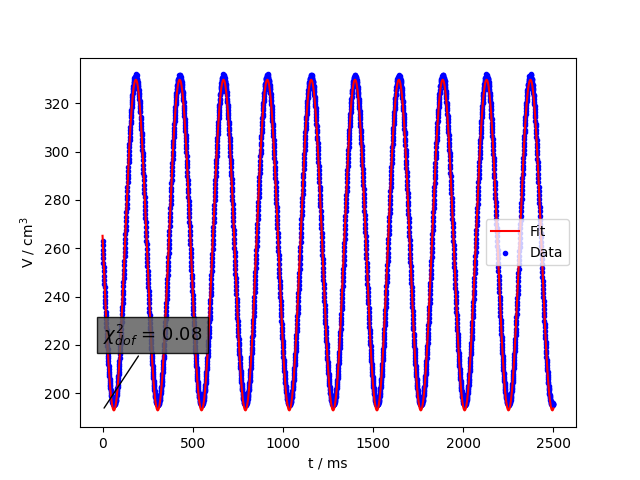
\includegraphics[width=.4\textwidth]{Unbelastet/fit_of_t_V.png}
    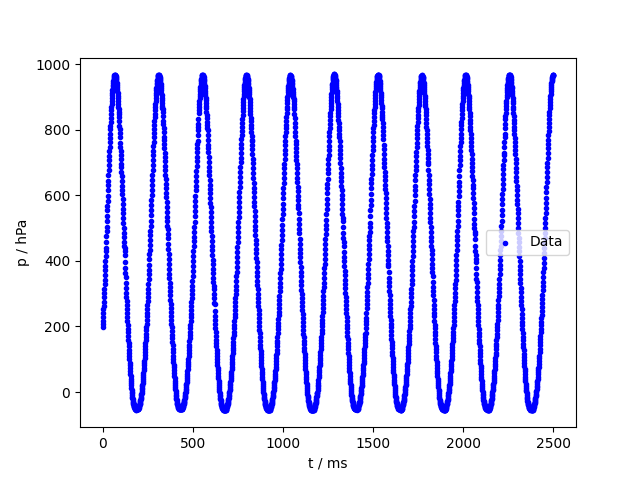
\includegraphics[width=.4\textwidth]{Unbelastet/fit_of_t_p.png}
    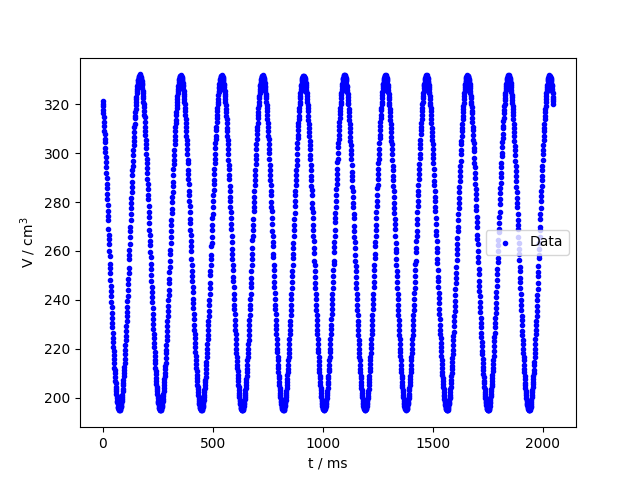
\includegraphics[width=.4\textwidth]{Belastet/fit_of_t_V.png}
    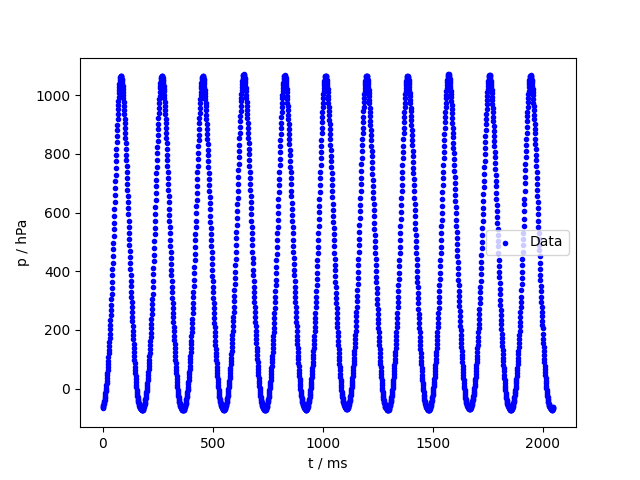
\includegraphics[width=.4\textwidth]{Belastet/fit_of_t_p.png}
    \caption{Links oben die $p(t)$ Daten und rechts oben die $V(t)$ Daten
    für den unbelasteten Motorbetrieb und links unten die $p(t)$ Daten 
    und rechts unten die $V(t)$ Daten für den belasteten Motorbetrieb
}%
    \label{fig:ptvtdaten}
\end{figure}
Um $P_{\text{mech}}$ zu bestimmen wird die zuvor ermittelte mechanische Arbeit
pro Zyklus $W_{\text{mech}}$ mit der Drehzahl $n$ multipliziert. Welche entweder
durch Abzählen der Perioden und der verstrichenen Zeit in den Daten oder
durch die Fourier-Analyse der Volumsschwingung 
$V(f) = \frac{1}{\sqrt{2\pi}^n} \int_{-\infty}^{\infty} V(t) e^{-ift} dx$
und herauslesen bei welcher Frequenz der Peak am höchsten ist, siehe 
\autoref{fig:fourier_unbelastet} und \autoref{fig:fourier_belastet}, 
bestimmt werden kann.

\begin{minipage}{\textwidth}
\begin{minipage}[t]{0.49\textwidth}
    \centering
    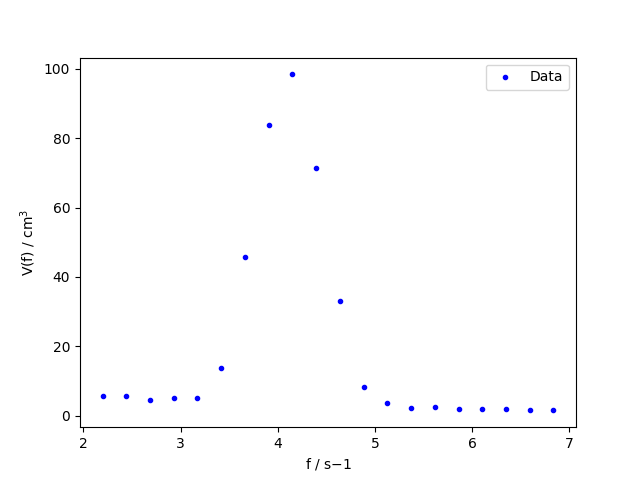
\includegraphics[width=\textwidth]{Unbelastet/fit_of_f_Vf.png}
    \captionbelowof{figure}{Fourier-Analyse des Stirlingmotors im unbelasteten Betrieb}
    \label{fig:fourier_unbelastet}
\end{minipage}
\begin{minipage}[t]{0.49\textwidth}
    \centering
    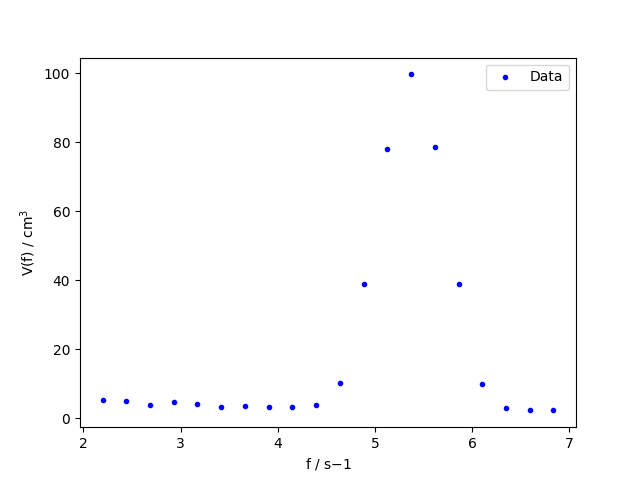
\includegraphics[width=\textwidth]{Belastet/fit_of_f_Vf.png}
    \captionof{figure}{Fourier-Analyse des Stirlingmotors im belasteten Betrieb}
    \label{fig:fourier_belastet}
\end{minipage}
    \vspace{1em}
\end{minipage}

Wie im ersten Bild, siehe \autoref{fig:ptvtdaten} ersichtlich wurde um 
die genaue Drehzahl zu bestimmen die Datenpunkte gefittet und haben foldende
Werte bekommen, siehe \autoref{tab:Drehzahl}. Damit die Daten noch sauber
zu sehen ist entschieden worden nur einen Fit in die Daten zu plotten.

\begin{table}[h]
    \centering
    \caption{Die Drehzahl $n_{\text{daten}}$ anhand den $p(t)$ und den $V(t)$ Daten.
        Die Drehzahl $n_{\text{fourier}}$ ermittelt durch die Auswertung der Fourier-tranformierten
    Daten.}
    \label{tab:Drehzahl}
    \begin{tabular}{c|S|S}
        Betriebsart: & $n_{\text{daten}}$               & $n_{\text{fourier}}$             \\ \hline
        Unbelastet     & \SI{4.112+-0.003}{\hertz} & \SI{4.10(10)}{\hertz} \\ \hline
        Belastet   & \SI{5.376+-0.003}{\hertz} & \SI{5.40(10)}{\hertz} \\ \hline
    \end{tabular}
\end{table}

Um die abgeführte Wärmeleistung $P_{\text{ab}}$ zu bestimmen, muss der Volumenstrom,
die Dichte von Wasser, die Temperaturerhöhung und die spezifische Wärmekapazität
von Wasser bekannt sein. Die Temperaturerhöhung wird mit zwei Thermometern
gemessen einmal beim Eingang des Stirlingmotors und einmal beim Ausgang.
Der Volumenstrom wurde gemessen, indem der Wasserstand zweimal mit
möglichst großen zeitlichen Abstand abgelesen. Nun wurde die benötigte Zeit
des Wassers, um den Messbecher bis zu diesem Wert zu füllen, mittels eines
Videobearbeitungsprogramm ermittelt. Es wurden die genauen Frames bestimmt, 
bei dem das Wasser 100 ml und 250 ml überschreitet. Mit den Timestamps der
Bilder ist das Zeitintervall, welches gebraucht wurde um 150 ml dem Gefäß 
hinzuzufügen, auf \SI{+-0.06}{\second} bestimmt.

\begin{table}[h]
    \centering
    \caption{Daten für die Berechnung des Volumenstroms}
    \label{tab:volumenstromdata}
    \begin{tabular}{c|S|S}
    
        Betriebsart: & $\Delta V$ & $\Delta t$ \\ \hline
        Belastet   & \SI{150.0+-0.10}{\ml} & \SI{36.7+-0.06}{\second} \\ \hline
        Unbelastet & \SI{150.0+-0.10}{\ml} & \SI{36.5+-0.06}{\second} \\ \hline
    \end{tabular}
\end{table}

Die spezifische Wärmekapazität wurde von dem Artikel \cite{uitspezifische} entnommen
und beträgt \SI{4187}{\joule\per\kilogram\per\kelvin}.
Die Dichte von Wasser wurde von der Website \cite{Wagner2002} entnommen und 
beträgt bei den hier wichtigen Temperaturen:

\begin{itemize}
    \item \SI{0.998599}{\gram\per\ml} @ \SI{18.0}{\celsius} 
    \item \SI{0.997518}{\gram\per\ml} @ \SI{23.1}{\celsius}
    \item \SI{0.997175}{\gram\per\ml} @ \SI{24.5}{\celsius}
    \item \SI{0.998207}{\gram\per\ml} @ \SI{20.0}{\celsius}
\end{itemize}

Zusätzliche ist noch die mechanische Leistung des belasteten Stirlingmotors
mittels dem Bremszaum und der Federwaage zu bestimmen. Da der Wert für
die Kraft $F$ sehr schwankte ist dieser nicht genauer ablesbar zeitliche
Mittelung dieser Daten wäre natürlich besser. Der Hebelarm $l$ hat eine Länge
von \SI{25+-0.5}{\cm} und die Kraft $F$ beträgt \SI{0.55(5)}{\newton}.

\section{Auswertung}
\label{sec:auswertung}

Kombinert man nun die Messwerte aus dem Kapitel \nameref{sec:versuchsdurchfuehrung_messergebnisse} 
mit den Gleichungen aus \nameref{sec:voraussetzungen_grundlagen}
kommt man auf die verschiedenen gesuchten Leistungen und Wirkungsgrade.

Wie schon in \nameref{sec:voraussetzungen_grundlagen} wurde für die Unsicherheitfortpflanzung 
die verallgemeinerte Gaußmethode verwendet und ist mittels Python \verb|scipy| ausgewertet
worden, zudem wurde auch großzügig gerundet.

Die $pV$ Diagramme sind auch visulisiert worden.

\begin{minipage}{\textwidth}
\begin{minipage}[t]{0.49\textwidth}
    \centering
    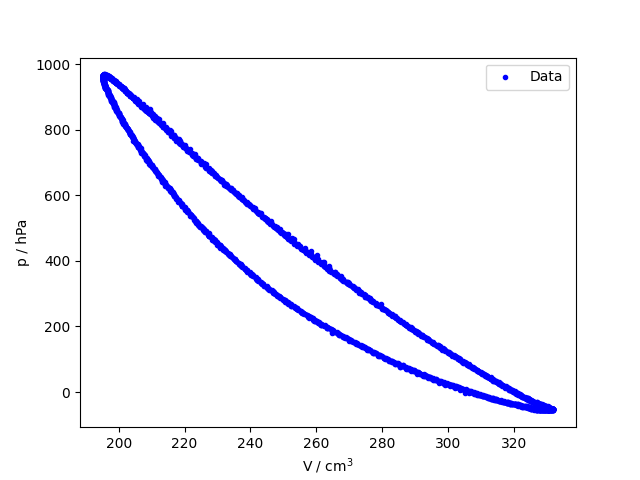
\includegraphics[width=\textwidth]{Unbelastet/fit_of_V_p.png}
    \captionbelowof{figure}{Das $pV$-Diagramm des Stirlingmotors im unbelasteten Betrieb}
    \label{fig:pVunbelastet}
\end{minipage}
\begin{minipage}[t]{0.49\textwidth}
    \centering
    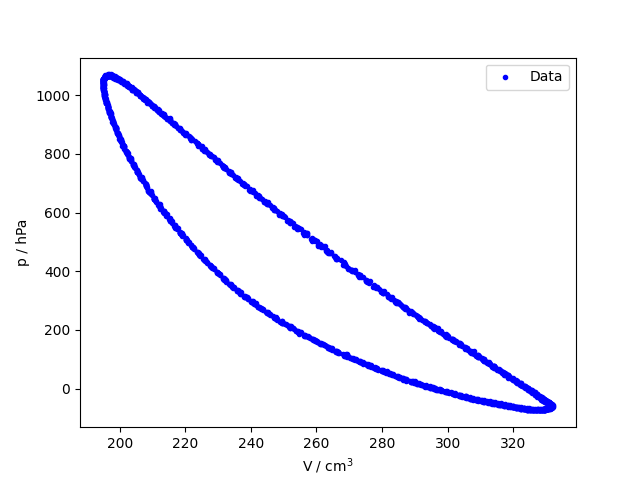
\includegraphics[width=\textwidth]{Belastet/fit_of_V_p.png}
    \captionof{figure}{Das $pV$-Diagramm des Stirlingmotors im belasteten Betrieb}
    \label{fig:pVbelastet}
\end{minipage}
    \vspace{1em}
\end{minipage}

Hier ist gut ersichtlich, wie eine höhere Temperaturquelle das $pV$-Diagramm
verändert. Die höher Temperaturquelle bewirkt wie erwartet, dass die Fläche unter 
der Kurve und somit die Leistung, welche an die Welle übertragen wird, größer wird.
Hier soll noch erwähnt werden, dass die Kanten im Vergleich zum Modell, welches
in den \nameref{sec:voraussetzungen_grundlagen} durchgemacht wurde, abgerundet sind.
Der Gründe dafür sind, dass keine Dichtung und keine Messung perfekt ist. Dadurch
wird ein Großteil der Abrundung erklärt, aber selbst wenn perfekte Messungen
und Dichtungen vorhanden wären, wären die Ecken leicht abgerundet, da Kanten,
also nicht Glatte Übergänge, unphysikalisch wären.

\begin{table}[H]
    \centering
    \caption{Die errechneten Leistungen und Wirkungsgrade und zusätzliche wichtige 
    Systemgrößen des Stirlingmotors. Genauer Beschreibungen der einzelnen
    Größen wurden, aus Gründen der besseren Übersichtlichkeit, in der Tabelle gemacht }
    \label{tab:leistungen_wirkungsgrade}
    \begin{tabular}{c|S[table-format=3.3(3)]|S[table-format=2.3(3)]|p{5cm}}
        {}                                             & $\text{Belastet}$ & $\text{Unbelastet}$ & Anmerkungen \\ \hline
        $P_{\text{0mech}} | P_{\text{L}}$ / W                 & 19.04(10)           & 7.69(10)              & Die Leistung bestimmt mittels numerischer Integration. \\
        $n_{\text{B}} | n_{\text{L}}$ / Hz                           & 4.112(3)          & 5.376(3)            & Die Drehzahlen von \autoref{tab:Drehzahl}. \\
        $\eta_{0} | \eta_{\text{L}}$ / \%                     & 7.72(10)            & 7.11(10)              & Der innere Wirkungsgrad bzw. Leerlauf Wirkungsgrad.  \\
        $P_{\text{mech}}$ / W                          & 4.6(6)            & {-}                 & Die Leistung die an die Antriebswelle abgebenen wird. \\
        $\eta_{\text{ges}}$ / \%                       & 1.9(3)            & {-}                 & Der Bruchteil(Wirkungsgrad) der von der hinzugefügten Leistung $P_{\text{elek}}$ in $P_{\text{mech}}$ umgewandelt wird. \\
        $P_{\text{ab}}$ / W                            & 111(2)            & 87(5)               & Die, über das Wasser abgeführte, Leistung. \\
        $Q_{\text{ab}}$  / J                           & 20.6(5)           & 21.3(5)             & Die, über das Wasser abgeführte, Wärmeenergie pro Zyklus. \\
        $\tilde{P}_{\text{0mech}} | \tilde{P}_{\text{L}}$ / W & 138(2)            & 20(5)               & Die Leistung, welche nicht an das Wasser übergeben wird, also $P_{\text{elek}}-P_{\text{ab}}$. \\
        $\tilde{\eta}_{0} | \tilde{\eta}_{\text{L}}$ / \%     & 55.4(8)           & 19(4)               & Der Bruchteil(Wirkungsgrad) der von der hinzuzufügen Leistung $P_{\text{elek}}$ in $\tilde{P}_{\text{0mech}}$ bzw. $\tilde{P}_{\text{L}}$ umgewandelt wird.\\
    \end{tabular}
\end{table}

\section{Diskussion und Zusammenfassung}
\label{sec:diskussion_zusammenfassung}
% %Aufzählung was scheiße glaufen is
Damit die Aufteilung der Energie besser verstanden werden kann sind zwei Diagramme
erstellt worden. Einmal für den belasteten und einmal für den unbelasteten 
Motorbetrieb, siehe \autoref{fig:aufteilung_unbelastet} und \autoref{fig:aufteilung_belastet}.
Die Heizleistung Leistung ($P_{\text{heiz}}$ oder auch $P_{\text{elek}}$ genannt) ist die gesamte 
Leistung, welche dem System hinzufügt wird. In diesen Diagrammen ist diese
die Zusammensetzung aller Teile des Kreises, also der ganze Kreis.

\begin{minipage}{\textwidth}
\begin{minipage}[t]{0.49\textwidth}
    \centering
    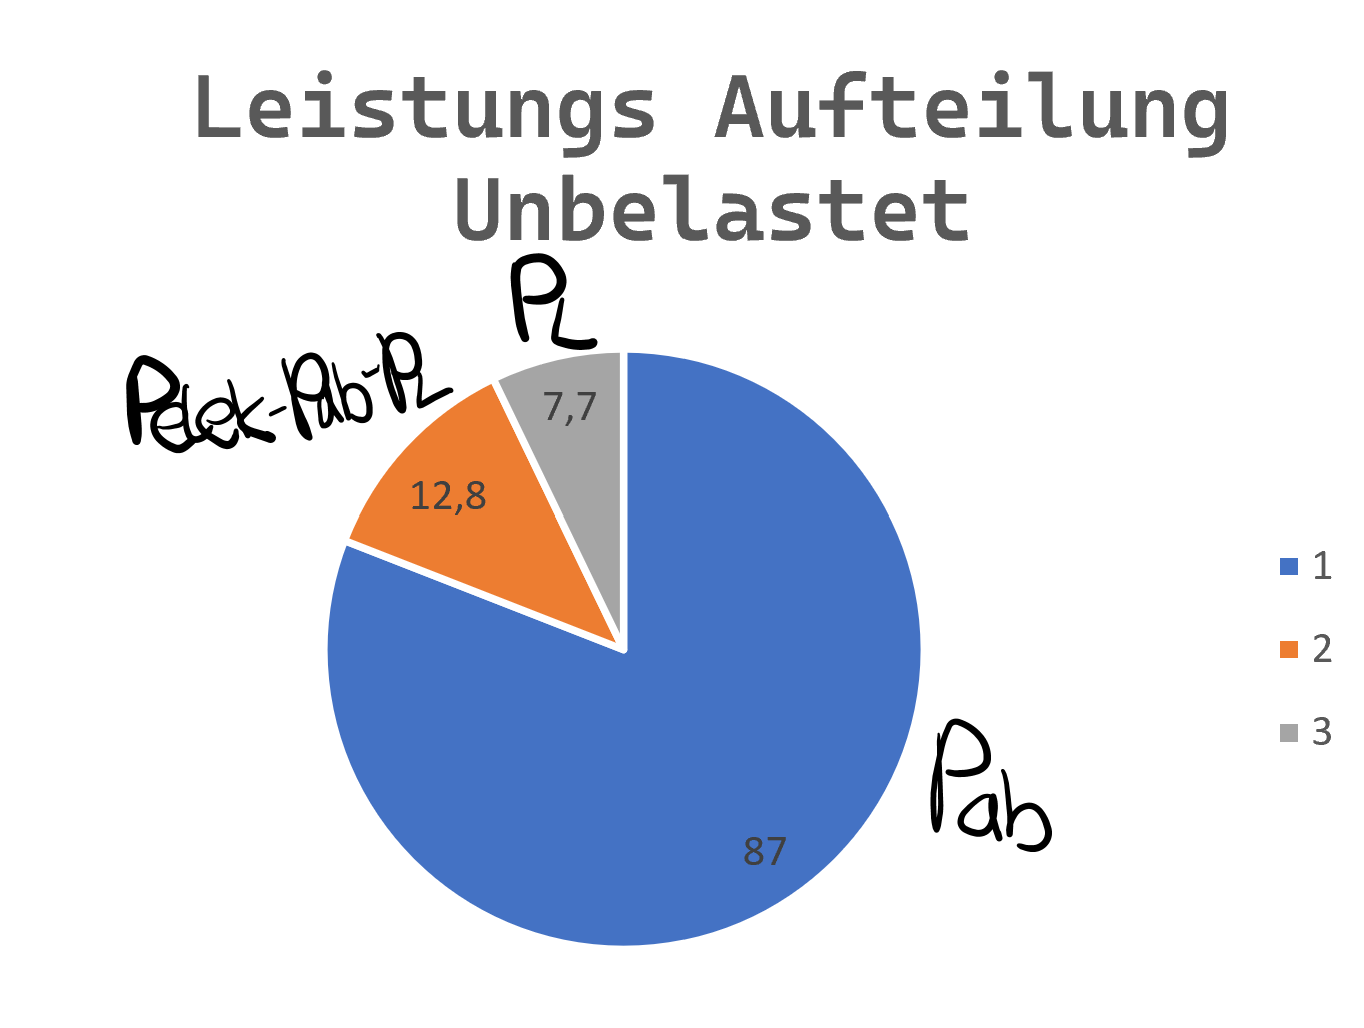
\includegraphics[width=\textwidth]{pics/leistungsaufteilungunbelastet.png}
    \captionbelowof{figure}{Die Aufteilung der hinzugefügten Leistung $P_{\text{elek}}$
        durch den unbelasteten Betrieb. Wobei $P_{\text{ab}}$ die abgeführte Leistung,
    $P_{\text{L}}$ die mechanische Leistung für die Deckung der inneren Verluste ist. 
    Der orange Teil des Kreis ist die Leistung, welche aus diversen Gründe an
    die Umgebung abgegeben wird.}
    \label{fig:aufteilung_unbelastet}
\end{minipage}
\begin{minipage}[t]{0.49\textwidth}
    \centering
    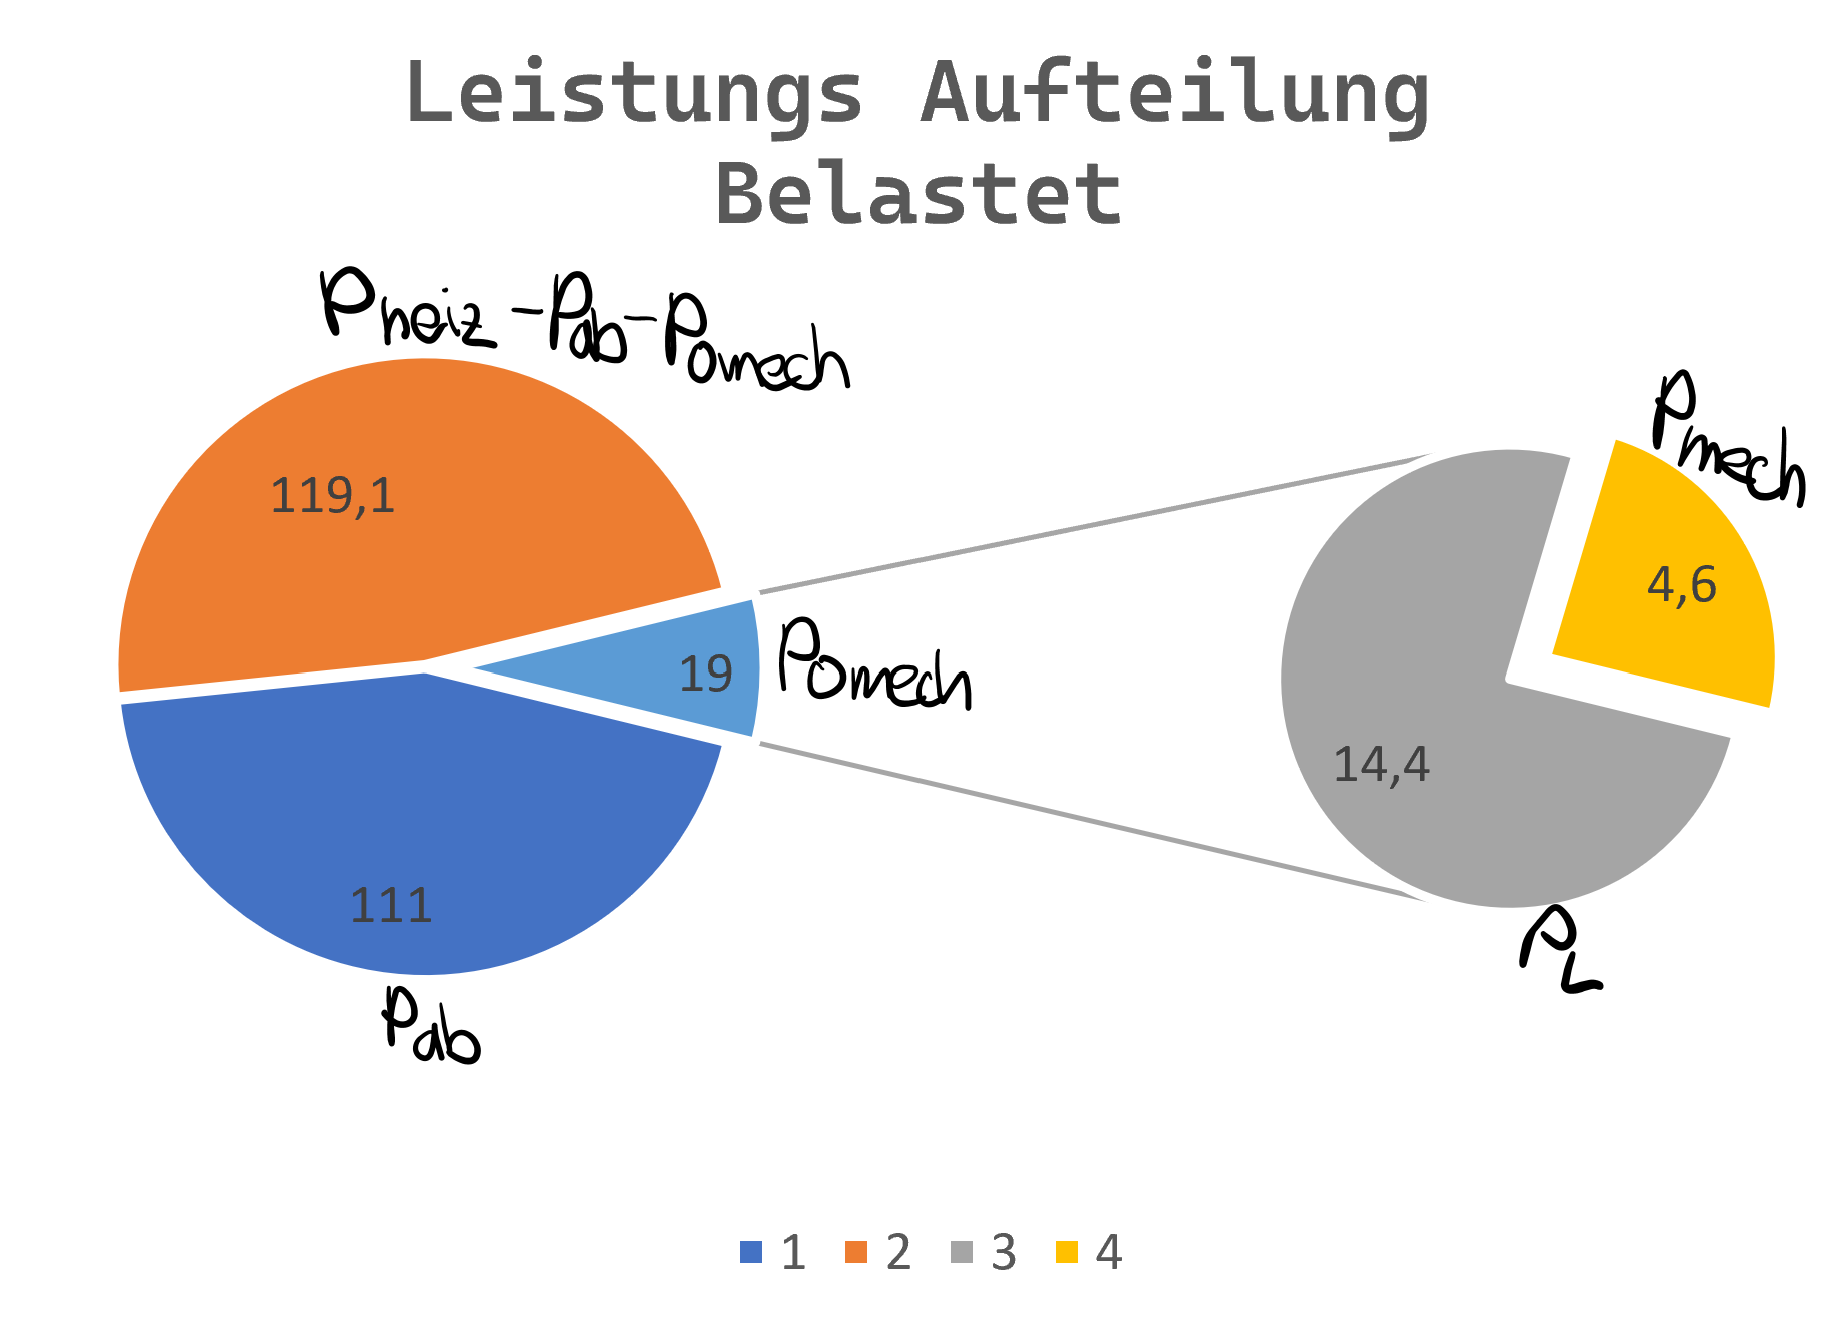
\includegraphics[width=\textwidth]{pics/leistungsaufteilungbelastet.png}
    \captionof{figure}{Die Aufteilung der hinzugefügten Leistung $P_{\text{elek}}$
        durch den belasteten Betrieb. Wobei $P_{\text{ab}}$ die abgeführte Leistung,
    $P_{\text{L}}$ die mechanische Leistung für die Deckung der inneren Verluste ist 
    und $P_{\text{mech}}$ die abgegriffene mechanische Leistung ist. 
    Der orange Teil des Kreis ist die Leistung, welche aus diversen Gründe an
    die Umgebung abgegeben wird.}
    \label{fig:aufteilung_belastet}
\end{minipage}
    \vspace{1em}
\end{minipage}

Die Diagramme und die Werte aus \autoref{tab:leistungen_wirkungsgrade} zeigen
uns, dass die Wirkungsgrade $\eta_{0}$ und $\eta_{\text{L}}$ größenordnungmäßig
übereinstimmen. Dies bedeutet, dass innere Wirkungsgrad das Equivalent zu dem
Leerlauf Wirkungsgrad vom unbelasteten Betrieb ist für den belasteten Betrieb.
Dies war auch erwartet da die Wirkungsgrade, obwohl die Leistungen
$P_{\text{0mech}}$ bzw. $P_{\text{L}}$ unterschiedlich groß sind, da
unterschiedlich viel Energie $P_{\text{elek}}$ ins System gesteckt wird,
großteils durch die Geometrie des Stirlingmotors gegeben sind. Natürlich wenn
die Temperaturdifferenz oder andere Grenzen des Stirlingmotors erreicht
unterscheiden sich diese Werte auch. 

Weiters zeigen die Diagramme auch, dass durch das Heizen ein größer Teil der
Leistung an die Umgebung weiter gegeben wird, in den Diagrammen orange dargestellt.

Wenn der Wirkungsgrad des gesamten Prozesses $\eta_{\text{ges}}$ gesteigert, werden
soll lässt sich aus den zovor erwähnten Punkte schließen, entweder die
Reibung verringert oder der Motor mehr isoliert werden muss.

Weiters ist es einfach anhand der Diagramme zusehen, dass $P_{\text{0mech}}$,
(bzw. $P_{\text{L}}$ beim unbelasteten Betrieb) nicht gleich den
$\tilde{P}_{\text{0mech}}$ bzw. $\tilde{P}_{\text{L}}$ sind. Somit
representieren sowohl deren Wirkungsgrade $\tilde{\eta}_{0}$ und
$\tilde{\eta}_{\text{L}}$ als auch deren Leistungen den orangen mit dem
$P_{\text{0mech}}$, (bzw. $P_{\text{L}}$ beim unbelasteten Betrieb)
kombinierten Anteil des Kreises. Also die mechanische Leistung mit den Abgaben
an die Umgebung. Daher ist auch die Vorgehensweiße die mechanische Leistung
$P_{\text{0mech}}$ (bzw.  $P_{\text{L}}$ beim unbelasteten Betrieb) mittels
Schlussrechnung ($P_{\text{0mech}} \stackrel{?}{=}
P_{\text{elek}}-P_{\text{ab}} = \tilde{P}_{\text{0mech}}$) zu bestimmen, hier
nicht sinnvoll ist, da eindeutigerweißer, wie in \autoref{fig:aufteilung_unbelastet} und
\autoref{fig:aufteilung_belastet} ersichtlich,  $P_{\text{0mech}} \neq
\tilde{P}_{\text{0mech}}$ ist.

Wenn die abgreifbare mechanische Leistung $P_{\text{mech}}$ genauer bestimmt werden
will sollte die Kraft $F$ über einen Sensor zeitlich aufgenommen werden und
über diese Daten gemittelt werden.

Bei den Drehzahlen konnte, durch das Fitten der Daten ein genauerer Wert für
die Drehzahl bestimmt werden. Jedoch beschreibt der, durchs Fitten erhaltene,
Wert nur unter der Annahme, dass die Schwingung perfekt periodisch ist, die
Drehzahl korrekt.  Diese Bedingung ist hier näherungweiße erfüllt. Ist die
Schwingung jedoch nicht perfekt periodisch, würde diese Methode die
Aperiodizität der Schwingung bei einem Sinusmodel nicht gut beschreiben.
Deshalb ist der, durch die Fourier-Analyse erhaltenen Daten, ermittelte Wert
eigentlich der physikalisch richtigere Wert, da dieser die Varianze der
einzelnen Schwingungen berücksichtig. Da jedoch nicht genug Messpunkte
aufgenommen worden, damit der FFT (Fast-Fourier-Transform) gegnügend Werte liefert, damit ein guter Wert
für die Drehzahl herauskommt ist in diesem Experiment der Drehzahlwert von dem
Fit verwendet worden.

Alle durch das Experiment erhaltenen Werte und Ergebnisse sind in
\autoref{tab:leistungen_wirkungsgrade} ersichtlich. 

Alles in allem konnte ein brauchbare Analyse eine Stirlingmotors gemacht
werden. Diese beinhaltet die Erstellung der genauen Leistungaufteilungen, der
zugeführten Leistung, im belasteten und unbelasteten Fall. Durch diese
Aufteilung wird ersichtlich, dass großteils der Leistung (\SI{47.81}{\percent})
beim belasteten Betrieb an die Umgebung abgegeben wird. Dies deutet
darauf hin, dass beim Optimieren der Motorleistung sich auf die 
thermische Isolierung des Motors sich fokusiert werden soll.

% Literaturtabelle
\newpage
\printbibliography

\listoffigures

\listoftables

\end{document}
